\section{Programming Methodologies} \label{sec:programming}

In this section we propose two programming methodologies targeted very differently. The fast MLC programming methodology is devised for ReRAM memory when performance is a very critical and seldom soft error can be tolerated. This assumption holds true for main memory in traditional memory hierarchy. DRAM-based main memory are usually designed with ECC to tackle particle-strike soft error. More importantly, most of the data in main memory does not have to be "stored" for a long time as either they will be updated frequently or they will be useless without future accesses. The reliable MLC programming methodology is more suitable for storage system where data integrity is extremely important. For example, the data in SSD or USB driver may need to be stored for years. Moreover, even microsecond-level write latency can be hidden by large block size in conventional NAND flash product, maintaining an acceptable bandwidth. We will use 3-bit MLC cell as illustrations in this section since 8-level stable states have been widely reported in experimental data for MLC ReRAM. We denote the three bits in a ReRAM cell as $D_2D_1D_0$ where $D_2$ is the most significant bit (MSB) and $D_0$ is the least significant bit (LSB). "111" denotes the lowest LRS resistance while "000" denotes the highest HRS resistance. 

\subsection{Fast MLC programming methodology}

\begin{figure}[t]
\centering
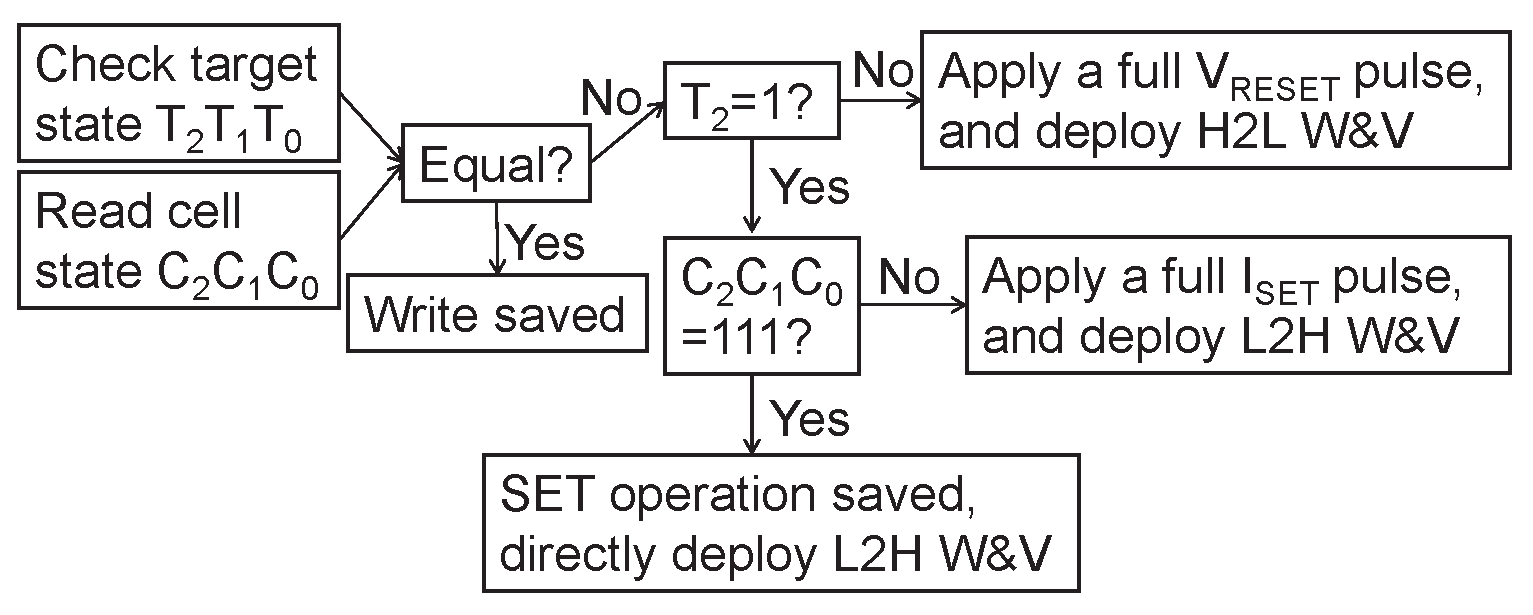
\includegraphics[width=0.48\textwidth]{fig/fastprog}
\vspace{-10pt}
\caption{Flowchart of fast programming methodology}
\label{fig:fastprog}
\vspace{-15pt}
\end{figure}

The goal of the fast MLC programming methodology is to reduce the average write latency by avoiding the states that require large number of iteration steps in either H2L or L2H programming. The flowchart of the proposed programming methodology is illustrated in Figure~\ref{fig:fastprog}.   


\subsection{Reliable MLC programming methodology}



